\documentclass[12pt,border=12pt]{standalone}
\usepackage[utf8]{inputenc}
\usepackage{tikz}
\usepackage{lmodern}
\usepackage{amsmath,amssymb}
\usetikzlibrary{shapes.geometric,arrows.meta,positioning,calc,fit,backgrounds,shadows}

\begin{document}
\fontsize{12pt}{15pt}\selectfont

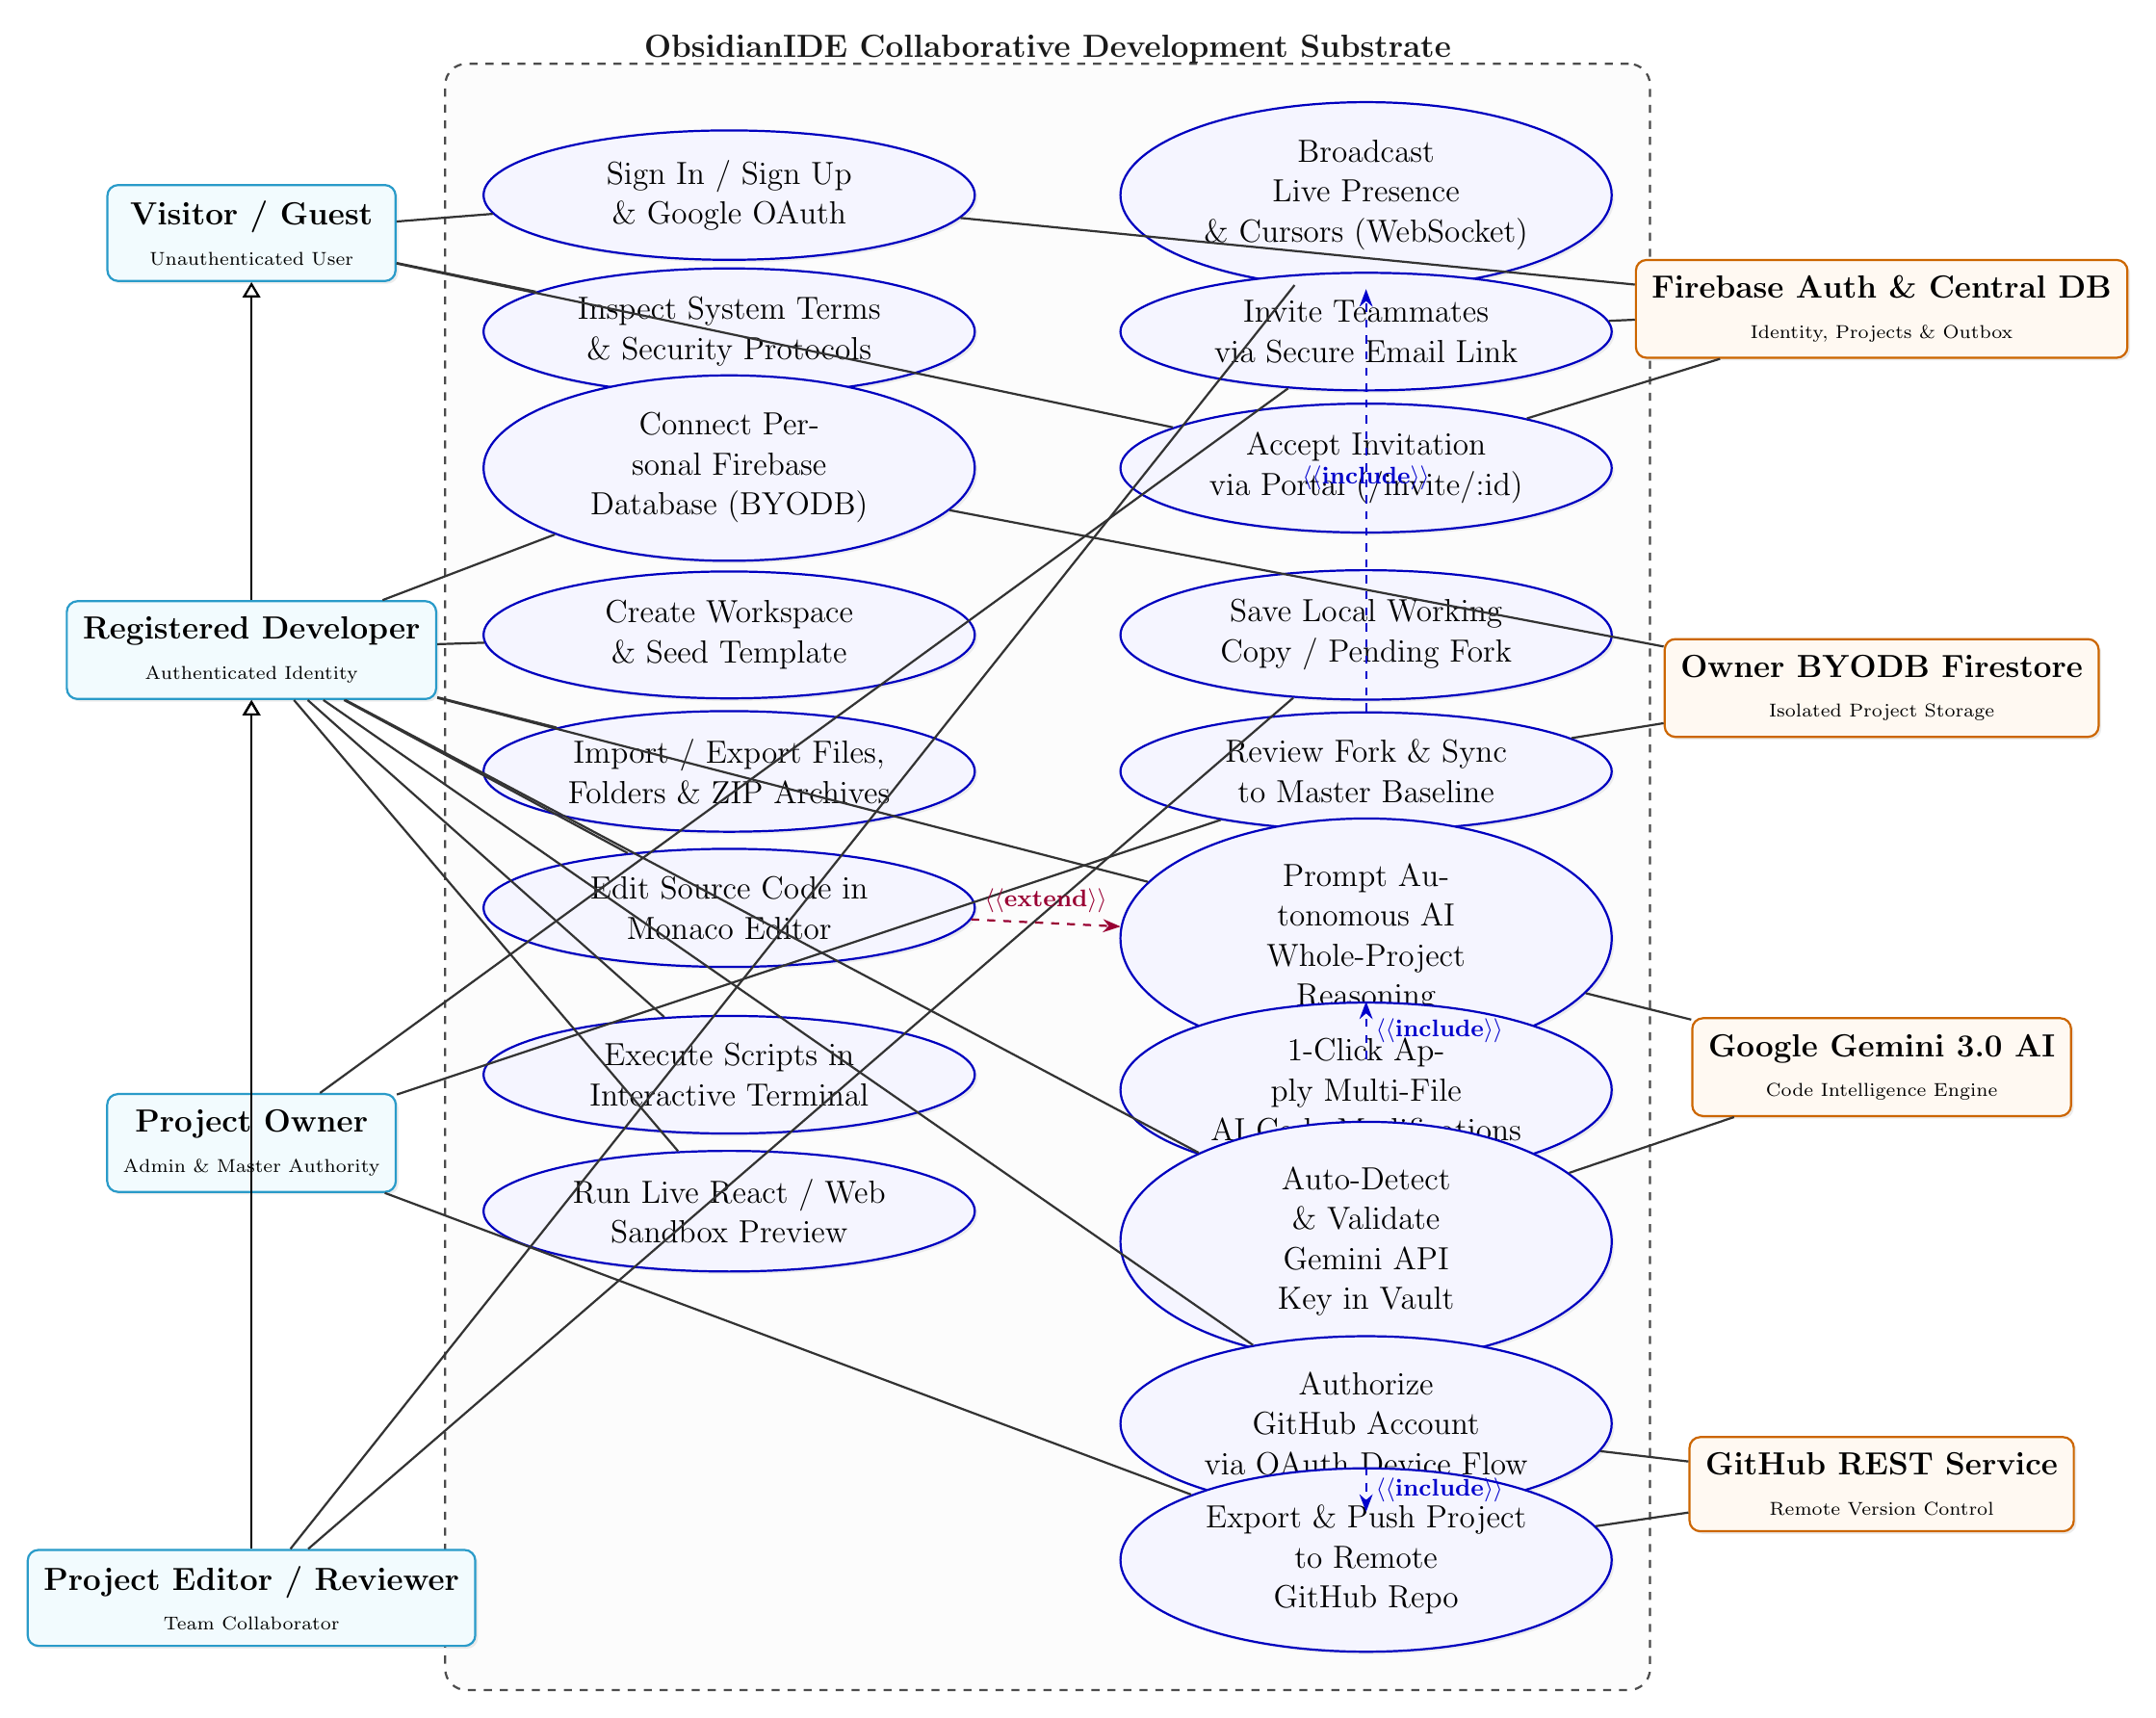
\begin{tikzpicture}[
    font=\fontsize{12pt}{15pt}\selectfont,
    >=Stealth,
    actor/.style={
        rectangle,
        draw=cyan!80!black,
        fill=cyan!5!white,
        thick,
        rounded corners=4pt,
        align=center,
        inner sep=6pt,
        minimum width=3.8cm,
        minimum height=1.2cm,
        drop shadow={opacity=0.15,shadow xshift=1pt,shadow yshift=-1pt}
    },
    systemActor/.style={
        rectangle,
        draw=orange!80!black,
        fill=orange!5!white,
        thick,
        rounded corners=4pt,
        align=center,
        inner sep=6pt,
        minimum width=4.0cm,
        minimum height=1.2cm,
        drop shadow={opacity=0.15,shadow xshift=1pt,shadow yshift=-1pt}
    },
    usecase/.style={
        ellipse,
        draw=blue!75!black,
        fill=blue!4!white,
        thick,
        align=center,
        inner sep=4pt,
        text width=4.3cm,
        minimum height=1.15cm,
        drop shadow={opacity=0.12,shadow xshift=1pt,shadow yshift=-1pt}
    },
    systemBoundary/.style={
        rectangle,
        draw=black!70,
        fill=gray!2!white,
        dashed,
        thick,
        rounded corners=8pt,
        inner sep=14pt
    },
    link/.style={
        thick,
        draw=black!80
    },
    includeLink/.style={
        dashed,
        thick,
        draw=blue!80!black,
        ->
    },
    extendLink/.style={
        dashed,
        thick,
        draw=purple!80!black,
        ->
    }
]

% ==================== LEFT ACTORS (HUMAN) ====================
\node[actor] (visitor) at (-10.5, 9.5) {\textbf{Visitor / Guest}\\\scriptsize Unauthenticated User};
\node[actor] (dev) at (-10.5, 4.0) {\textbf{Registered Developer}\\\scriptsize Authenticated Identity};
\node[actor] (owner) at (-10.5, -2.5) {\textbf{Project Owner}\\\scriptsize Admin \& Master Authority};
\node[actor] (editor) at (-10.5, -8.5) {\textbf{Project Editor / Reviewer}\\\scriptsize Team Collaborator};

% Actor Inheritance Hierarchy
\draw[thick, -{Triangle[open,scale=1.2]}] (dev) -- (visitor);
\draw[thick, -{Triangle[open,scale=1.2]}] (owner) -- (dev);
\draw[thick, -{Triangle[open,scale=1.2]}] (editor) -- (dev);

% ==================== SYSTEM BOUNDARY & USE CASES ====================

% Column 1: Auth, Project & Editing
\node[usecase] (ucAuth) at (-4.2, 10.0) {Sign In / Sign Up\\\& Google OAuth};
\node[usecase] (ucTerms) at (-4.2, 8.2) {Inspect System Terms\\\& Security Protocols};
\node[usecase] (ucBYODB) at (-4.2, 6.4) {Connect Personal Firebase\\Database (BYODB)};

\node[usecase] (ucCreateProj) at (-4.2, 4.2) {Create Workspace\\\& Seed Template};
\node[usecase] (ucFileIO) at (-4.2, 2.4) {Import / Export Files,\\Folders \& ZIP Archives};
\node[usecase] (ucEditCode) at (-4.2, 0.6) {Edit Source Code in\\Monaco Editor};

\node[usecase] (ucTerminal) at (-4.2, -1.6) {Execute Scripts in\\Interactive Terminal};
\node[usecase] (ucSandbox) at (-4.2, -3.4) {Run Live React / Web\\Sandbox Preview};

% Column 2: Collaboration, AI & Version Control
\node[usecase] (ucPresence) at (4.2, 10.0) {Broadcast Live Presence\\\& Cursors (WebSocket)};
\node[usecase] (ucInvite) at (4.2, 8.2) {Invite Teammates\\via Secure Email Link};
\node[usecase] (ucAcceptInvite) at (4.2, 6.4) {Accept Invitation\\via Portal (/invite/:id)};

\node[usecase] (ucSaveFork) at (4.2, 4.2) {Save Local Working\\Copy / Pending Fork};
\node[usecase] (ucSyncMaster) at (4.2, 2.4) {Review Fork \& Sync\\to Master Baseline};

\node[usecase] (ucAiChat) at (4.2, 0.2) {Prompt Autonomous AI\\Whole-Project Reasoning};
\node[usecase] (ucAiPatch) at (4.2, -1.8) {1-Click Apply Multi-File\\AI Code Modifications};
\node[usecase] (ucAiKey) at (4.2, -3.8) {Auto-Detect \& Validate\\Gemini API Key in Vault};

\node[usecase] (ucGitHubAuth) at (4.2, -6.2) {Authorize GitHub Account\\via OAuth Device Flow};
\node[usecase] (ucGitHubPush) at (4.2, -8.0) {Export \& Push Project\\to Remote GitHub Repo};

% ==================== RIGHT ACTORS (SYSTEMS) ====================
\node[systemActor] (fbAuth) at (11.0, 8.5) {\textbf{Firebase Auth \& Central DB}\\\scriptsize Identity, Projects \& Outbox};
\node[systemActor] (byodb) at (11.0, 3.5) {\textbf{Owner BYODB Firestore}\\\scriptsize Isolated Project Storage};
\node[systemActor] (geminiAI) at (11.0, -1.5) {\textbf{Google Gemini 3.0 AI}\\\scriptsize Code Intelligence Engine};
\node[systemActor] (githubAPI) at (11.0, -7.0) {\textbf{GitHub REST Service}\\\scriptsize Remote Version Control};

% ==================== SYSTEM BOUNDARY BOX ====================
\begin{scope}[on background layer]
    \node[systemBoundary, fit=(ucAuth) (ucTerms) (ucBYODB) (ucCreateProj) (ucFileIO) (ucEditCode) (ucTerminal) (ucSandbox) (ucPresence) (ucInvite) (ucAcceptInvite) (ucSaveFork) (ucSyncMaster) (ucAiChat) (ucAiPatch) (ucAiKey) (ucGitHubAuth) (ucGitHubPush), label={[font=\fontsize{13pt}{16pt}\selectfont\bfseries, text=black!90, yshift=-4pt]north:ObsidianIDE Collaborative Development Substrate}] (sysBox) {};
\end{scope}

% ==================== ASSOCIATIONS (ACTORS TO USE CASES) ====================

% Visitor associations
\draw[link] (visitor) -- (ucAuth);
\draw[link] (visitor) -- (ucTerms);
\draw[link] (visitor) -- (ucAcceptInvite);

% Developer associations
\draw[link] (dev) -- (ucBYODB);
\draw[link] (dev) -- (ucCreateProj);
\draw[link] (dev) -- (ucFileIO);
\draw[link] (dev) -- (ucEditCode);
\draw[link] (dev) -- (ucTerminal);
\draw[link] (dev) -- (ucSandbox);
\draw[link] (dev) -- (ucAiChat);
\draw[link] (dev) -- (ucAiKey);
\draw[link] (dev) -- (ucGitHubAuth);

% Owner associations
\draw[link] (owner) -- (ucInvite);
\draw[link] (owner) -- (ucSyncMaster);
\draw[link] (owner) -- (ucGitHubPush);

% Editor associations
\draw[link] (editor) -- (ucSaveFork);
\draw[link] (editor) -- (ucPresence);

% System Actor Associations
\draw[link] (ucAuth) -- (fbAuth);
\draw[link] (ucInvite) -- (fbAuth);
\draw[link] (ucAcceptInvite) -- (fbAuth);
\draw[link] (ucSyncMaster) -- (byodb);
\draw[link] (ucBYODB) -- (byodb);
\draw[link] (ucAiChat) -- (geminiAI);
\draw[link] (ucAiKey) -- (geminiAI);
\draw[link] (ucGitHubAuth) -- (githubAPI);
\draw[link] (ucGitHubPush) -- (githubAPI);

% ==================== INCLUDE & EXTEND RELATIONSHIPS ====================
\draw[includeLink] (ucAiChat) -- node[right, font=\fontsize{9pt}{11pt}\selectfont\bfseries, text=blue!80!black] {$\langle\langle\text{include}\rangle\rangle$} (ucAiPatch);
\draw[includeLink] (ucGitHubPush) -- node[right, font=\fontsize{9pt}{11pt}\selectfont\bfseries, text=blue!80!black] {$\langle\langle\text{include}\rangle\rangle$} (ucGitHubAuth);
\draw[extendLink] (ucEditCode) -- node[above, font=\fontsize{9pt}{11pt}\selectfont\bfseries, text=purple!80!black] {$\langle\langle\text{extend}\rangle\rangle$} (ucAiChat);
\draw[includeLink] (ucSyncMaster) -- node[above, font=\fontsize{9pt}{11pt}\selectfont\bfseries, text=blue!80!black] {$\langle\langle\text{include}\rangle\rangle$} (ucPresence);

\end{tikzpicture}
\end{document}
